\chapter{Pump linearization and PI controller}
\label{cha:linear_pump}

The control structure chosen in \chapref{control_problem} and shown in \figref{fig:control_structure} includes a PI controller, which is to designed. The PI controllers purpose is to use the optimized control output from the MPC as a control reference. 

The control focus of this project has been on the model predictive control, see \secref{sec:MPC}. Therefore a simple PI controller has been design, where the control structure can be seen on \figref{fig:simple_PI}.

\begin{figure}[H]
\centering
\begin{tikzpicture} [scale=0.8,transform shape]

\draw  (2.5,1) rectangle (4.5,0);
\node at (3.5,0.5) {G(s)};

\draw  (-1,1) rectangle (1,0);
\node at (0,0.5) {D(s)};

\draw[-triangle 60] (-3,0.5) -- (-1,0.5);
\draw[-triangle 60] (4.5,0.5) -- (6,0.5);
\draw[-triangle 60] (1,0.5) -- (2.5,0.5);
\draw[-triangle 60] (-5,0.5) -- (-3.5,0.5);
%\draw[-triangle 60] (-5.5,0.5) -- (-4.5,0.5);

\draw[-triangle 60] (5.25,0.5) -- (5.25,-1) -- (-3.25,-1) -- (-3.25,0.25);

%\node at (-5.5,1) {$CP_{ref}$};
\node at (-5,0.75) {$\Delta P_{ref}$};
\node at (-2.1,0.75) {$\Delta P_{error}$};
\node at (-3.75,0.8) {\large{$+$}};
\node at (-3.6,-0.08) {\large{$-$}};
\node at (5.25,0.75) {$\Delta p$};
\node at (1.75,0.75) {\large{$\omega$}};

\draw  (-3.25,0.5) ellipse (0.25 and 0.25);
\end{tikzpicture}%
  
\caption{The structure of the PI controller.}
\label{fig:simple_PI}
\end{figure}

The output from the MPC is a differential pressure, which is to be controlled through the rotational speed of the pumps. The general model for the pumps is given from \eqref{eq:PumpModel} as 

\begin{equation*}
\Delta p = -a_{h2}{q_i}^2 + a_{h1} \omega_r q_i + a_{h0}{\omega_r}^2
\end{equation*}

which is a nonlinear model. By the assumption that the flow is constant, the expression can through a Taylor expansion be linearized, with respect to $\omega$, to a small signal model.


For simplification the pump model is separated into smaller chunks, see \eqref{eq:tay_1}, then Taylor approximated, see \eqref{eq:tay_2}, where $\omega = \hat{\omega}+\bar{\omega}$.

\begin{equation}
\begin{split}
f_1(\bar{\omega}) &= a_{h1}\bar{q}\bar{\omega} \\
f_2(\bar{\omega}) &= a_{h0}\bar{\omega}^2
\end{split}
\label{eq:tay_1}
\end{equation}


\begin{equation}
\begin{split}
f_{t1}(\omega) &= f_1(\bar{\omega}) + f_1'(\bar{\omega})\cdot(\omega - \hat{\omega}) \\
f_{t2}(\omega) &= f_2(\bar{\omega}) + f_2'(\bar{\omega})\cdot(\omega - \hat{\omega})
\end{split}
\label{eq:tay_2}
\end{equation}

From \eqref{eq:tay_1} an expression for the workspace of, $\bar{\Delta P}$, can be made.

\begin{equation}
\begin{split}
\bar{\Delta P} = f_{1}(\bar{\omega}) + f_{2}(\bar{\omega}) + c
\end{split}
\label{eq:tay_3}
\end{equation}

The linear pump model can then be expressed as seen in \eqref{eq:tay_4}

\begin{equation}
\begin{split}
0 &= -(\bar{\Delta P} + \hat{\Delta P}) + f_{t1}(\bar{\omega}) + f_{t2}(\bar{\omega}) + c\\
  &= -(f_{1}(\bar{\omega}) + f_{2}(\bar{\omega}) + c + \hat{\Delta P}) + f_{t1}(\bar{\omega}) + f_{t2}(\bar{\omega}) + c \\ 
  &= -\hat{\Delta P} + f_1'(\bar{\omega})\cdot\hat{\omega} + f_2'(\bar{\omega})\cdot\hat{\omega}
\end{split}
\label{eq:tay_4}
\end{equation}

\eqref{eq:tay_4} is then Laplace transformed and solved for the input output relationship as seen on \figref{fig:simple_PI}

\begin{equation}
G(s) = \frac{\Delta P}{\omega} = f'_1(\bar{\omega}) + f'_2(\bar{\omega}) = a_{h1}\bar{q} + 2a_{h0}\bar{\omega}
\label{eq:lin_pump_simon}
\end{equation}

With the following operating points set for the pumps, the differential pressure over the pumps and their respective valves are measured. 

\begin{equation}
\centering
	\begin{split}
	\omega_{C18} &= 0.16,\hspace{20pt} \Delta P_{C18} = 0.0807 \\
	\omega_{C25} &= 0.4,\hspace{20pt} \Delta P_{C25} = 0.255  \\
	\omega_{C2}  &= 0.4,\hspace{20pt} \Delta P_{C2} = 0.2 \\
	\omega_{C16} &= 0.4,\hspace{20pt} \Delta P_{C16} =0.25 
	\end{split}
\end{equation}

From this the flow through the pumps can be estimated through \eqref{omega_notzero}, with their respective pump parameters found in \appref{system_description}.
\begin{equation}
\begin{split}
q_{C18} &= 0.179 \\
q_{C25} &= 0.272 \\
q_{C2} &= 0.061 \\
q_{C16} &= 0.169
\end{split}
\end{equation}

By inserting the values for the linearized model in \eqref{eq:lin_pump_simon}, the final models ends up as gains. 

\begin{equation}
	\begin{split}
	G_{C18}(s) &= 0.218 \\
	G_{C25}(s) &= 0.548 \\
	G_{C2}(s) &= 0.962 \\
	G_{C16}(s) &= 0.963
	\end{split}
\end{equation}


By using the Matlab design tool box for dynamical systems and having the settling time of 4 seconds in mind, the gains for the PI controller can be found as shown in \eqref{eq:PI_GAINS}. The step response of the pump PI system can be seen on \figref{fig:Tikz_PI_PUMP_GAIN}.
\begin{equation}
	\begin{split}
	K_{C18} &= 8 \\
	K_{C25} &= 3 \\
	K_{C2} &= 2 \\
	K_{C16} &= 2
	\end{split}
	\label{eq:NEW_PI_GAINS}
\end{equation}

% \begin{figure}[H]
% \centering
% % This file was created by matlab2tikz.
%
%The latest updates can be retrieved from
%  http://www.mathworks.com/matlabcentral/fileexchange/22022-matlab2tikz-matlab2tikz
%where you can also make suggestions and rate matlab2tikz.
%
\definecolor{mycolor1}{rgb}{0.00000,0.44700,0.74100}%
%
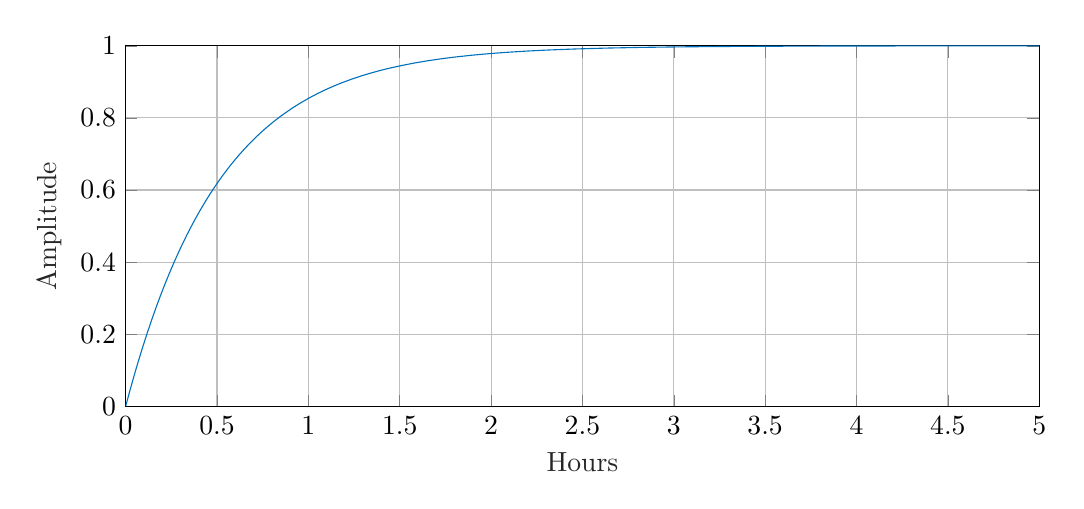
\begin{tikzpicture}

\begin{axis}[%
width=4.568in,
height=1.803in,
at={(0.766in,0.486in)},
scale only axis,
xmin=0,
xmax=5,
xlabel style={font=\color{white!15!black}},
xlabel={Hours},
ymin=0,
ymax=1,
ylabel style={font=\color{white!15!black}},
ylabel={Amplitude},
axis background/.style={fill=white},
xmajorgrids,
ymajorgrids
]

\addplot [color=mycolor1, forget plot]
  table[row sep=crcr]{%
0	0\\
0.0239225439509072	0.045007413978559\\
0.0478450879018153	0.0879891606440806\\
0.0717676318527225	0.129036410043906\\
0.0956901758036306	0.168236228897311\\
0.119612719754538	0.205671765275698\\
0.143535263705446	0.241422424970792\\
0.167457807656353	0.275564039924983\\
0.19138035160726	0.308169029081034\\
0.215302895558168	0.339306551992372\\
0.239225439509076	0.369042655519773\\
0.263147983459984	0.397440413925607\\
0.287070527410891	0.424560062662806\\
0.310993071361799	0.450459126142338\\
0.334915615312706	0.475192539750188\\
0.358838159263613	0.498812766372688\\
0.382760703214521	0.521369907677321\\
0.406683247165429	0.542911810385084\\
0.430605791116337	0.563484167759793\\
0.454528335067244	0.583130616529623\\
0.478450879018152	0.60189282944646\\
0.502373422969059	0.619810603679396\\
0.526295966919966	0.636921945229856\\
0.550218510870875	0.653263149547426\\
0.574141054821782	0.668868878517366\\
0.59806359877269	0.68377223398312\\
0.621986142723597	0.698004827959757\\
0.645908686674505	0.711596849687298\\
0.669831230625412	0.724577129666142\\
0.69375377457632	0.736973200810422\\
0.717676318527228	0.748811356849002\\
0.741598862478135	0.760116708098011\\
0.765521406429043	0.770913234723183\\
0.78944395037995	0.781223837605006\\
0.813366494330858	0.791070386914558\\
0.837289038281765	0.800473768503075\\
0.861211582232673	0.809453928203639\\
0.909056670134488	0.826219917125028\\
0.956901758036303	0.841510680753855\\
1.00474684593812	0.855456022925375\\
1.05259193383993	0.868174326144328\\
1.10043702174175	0.879773556538229\\
1.14828210964356	0.890352180385653\\
1.19612719754538	0.899999999999974\\
1.24397228544719	0.908798916064383\\
1.29181737334901	0.916823622889709\\
1.33966246125082	0.924142242497059\\
1.38750754915264	0.930816902908085\\
1.43535263705446	0.93690426555196\\
1.50712026890718	0.945045912614219\\
1.5788879007599	0.952136990767719\\
1.65065553261262	0.958313061652951\\
1.72242316446535	0.963692194522975\\
1.79419079631807	0.968377223398304\\
1.8898809721217	0.973697320081035\\
1.98557114792533	0.978122383760494\\
2.08126132372896	0.981802991413891\\
2.2008740434835	0.985545602292533\\
2.32048676323804	0.988518463785025\\
2.46402202694348	0.991290364100434\\
2.63147983459983	0.993690426555194\\
2.82286018620709	0.995634841677595\\
3.06208562571617	0.99724577129666\\
3.37307869707797	0.998486438751562\\
3.80368448819431	0.999339306551992\\
4.49743826277063	0.999826219917124\\
5.02373422969059	0.999936904265551\\
};
\end{axis}


\end{tikzpicture}%
% \caption{Step response of the pump PI system.}
% \label{fig:Tikz_PI_PUMP_GAIN}
% \end{figure}

\subsection*{PI test}

The PI controller was implemented on the water system described in \chapref{system_overview}. From the test it where concluded that some tuning of the gains had to be done, due to large overshoots and marginal stabilities on some of the pumps. The final values where found by trail and errors and can be seen in \eqref{eq:NEW_PI_GAINS}. 

\begin{equation}
	\begin{split}
	K_{C18} &= 6 \\
	K_{C25} &= 4 \\
	K_{C2} &= 1.4 \\
	K_{C16} &= 1.4
	\end{split}
	\label{eq:NEW_PI_GAINS}
\end{equation}

Whit these gains the systems gets a slower response than the settling time of 4 seconds. However this is still deemed fit to this project, since dynamics of the WT is much slower.